\mode<beamer>{
\usetheme{Berkeley}
%\usetheme{Frankfurt}
\setbeamertemplate{navigation symbols}{}
}
\mode<handout>{
\usepackage{pgfpages}
\pgfpagesuselayout{4 on 1}[a4paper, border shrink=10mm, landscape]
\usetheme{default}
}



% \setbeamertemplate{footline}{\hspace{3cm}
% Jeromy Anglim (\url{jeromyanglim.blogspot.com}) - 
% Melbourne R User Group\hfill\insertframenumber }

\usepackage[overlay, absolute]{textpos}


\title{Reproducible Research and R Workflow}
\subtitle{Melboure R Users Group (melbURN)}
\author{Jeromy Anglim}
\institute{Psychological Sciences, University of Melbourne}
\date{1st December 2010}

\begin{document} 
\mode*
\section{Introduction}
\begin{frame}
\titlepage
\begin{center}
	\url{jeromyanglim.blogspot.com}
\end{center}
\end{frame}

\begin{frame}
\frametitle{Outline}
\tableofcontents
\end{frame}

\begin{frame}{Quote from John Chanmbers}

\begin{quote}
The Mission:\\ 
Enable the best and most thorough exploration of data possible.

...

The Prime Directive:\\
The computations and the software for data analysis should be trustworthy.
\end{quote}

\tiny{Source: John M. Chambers,
Chapter 1, \emph{Software For Data Analysis: Programming with R}}
\end{frame}

\begin{frame}{What is the End Product?}
\begin{itemize}
\item Report
	\begin{itemize}
	  \item Console displayed versus no console displayed 
	  \item Batch versus once off
	\end{itemize}     
\item Data: 
	\begin{itemize}
  	  \item Cleaned
	  \item Processed
	  \item Documented
    \end{itemize}
\item Data anlysis software: 
	\begin{itemize}
	  \item R Package
	  \item A model 
	\end{itemize}
\end{itemize}

\begin{block}{Focus of this talk}
\begin{itemize}
  \item A workflow for writing reproducible data driven reports
\end{itemize}
\end{block}
\end{frame}


\begin{frame}{The Initial Challenge for the R Learner}
\begin{block}{How should you}
\begin{itemize}
\item  divide a project into files and folders?
\item incorporate R analyses into a report?
\item convert default R output into publication quality 
  tables, figures, and text?
\item build the final product?
\item sequence the analyses?
\item divide code into functions?
\end{itemize}
\end{block}
i.e., How do you efficiently achieve the Mission and fulfill the Prime Directive?
\end{frame}


\section{Workflow}
\begin{frame}{David Smith's Tips on R Workflow}
\begin{itemize}
  \item \emph{Transparency}: 
  	Logical organisation of units
  \item \emph{Maintanability}: 
  	Standardisation, clear comments
  \item \emph{Modularity}: 
  	DRY Principle, Discrete units
  \item \emph{Portability}: 
  Relative paths, minimise dependencies, dependencies are clear
  \item \emph{Reproducibility}: 
  Easy to reproduce results
  \item \emph{Efficiency}: 
  Easy to maintain and modify
\end{itemize}


{\tiny Source: \url{http://blog.revolutionanalytics.com/2010/10/a-workflow-for-r.html}}
\end{frame}

\begin{frame}{Josh Reisch LCFD Model}
\begin{enumerate}
\item load.R
\item clean.R
\item func.R
\item do.R 
\end{enumerate} 

{ \tiny Source: 
\url{http://stackoverflow.com/questions/1429907/workflow-for-statistical-analysis-and-report-writing/1434424}}

\end{frame}
 
\begin{frame}[containsverbatim]{John Myles White and ProjectTemplate}
\begin{block}{Best practice ideas}
\begin{itemize}
  \item Efficient creation of new projects
  \item Standardised folder and file structure 
  (i.e., \verb+data, diagnostics, doc, graphs, lib,+
  \verb+logs, profiling, reports, tests+) 
  \item Automatic data loading
  \item README and TODO files
  \item Encourages unit testing
  \item Standardised location of \verb+library()+ statements
  \item and more \ldots 
\end{itemize} 
\end{block}
\end{frame}


\begin{frame}[containsverbatim]{ProjectTemplate}
\begin{verbatim}
install.packages('ProjectTemplate')
library('ProjectTemplate')
?ProjectTemplate

create.project('my-project')

setwd('my-project')

load.project()
\end{verbatim} 

{\tiny See also 
 \url{http://www.johnmyleswhite.com/notebook/2010/08/26/projecttemplate/}}
\end{frame}


  

\section{Tools}
\subsection{Eclipse and StatET}
\begin{frame}{R Programming Environments}
\begin{itemize}
\item Rgui
\item Emacs + ESS
\item Eclipse + StatET
\item Any text editor + command line
\item and many more \ldots
\end{itemize}
\end{frame}

\begin{frame}{Eclipse and StatET: Screenshot}
\begin{center}
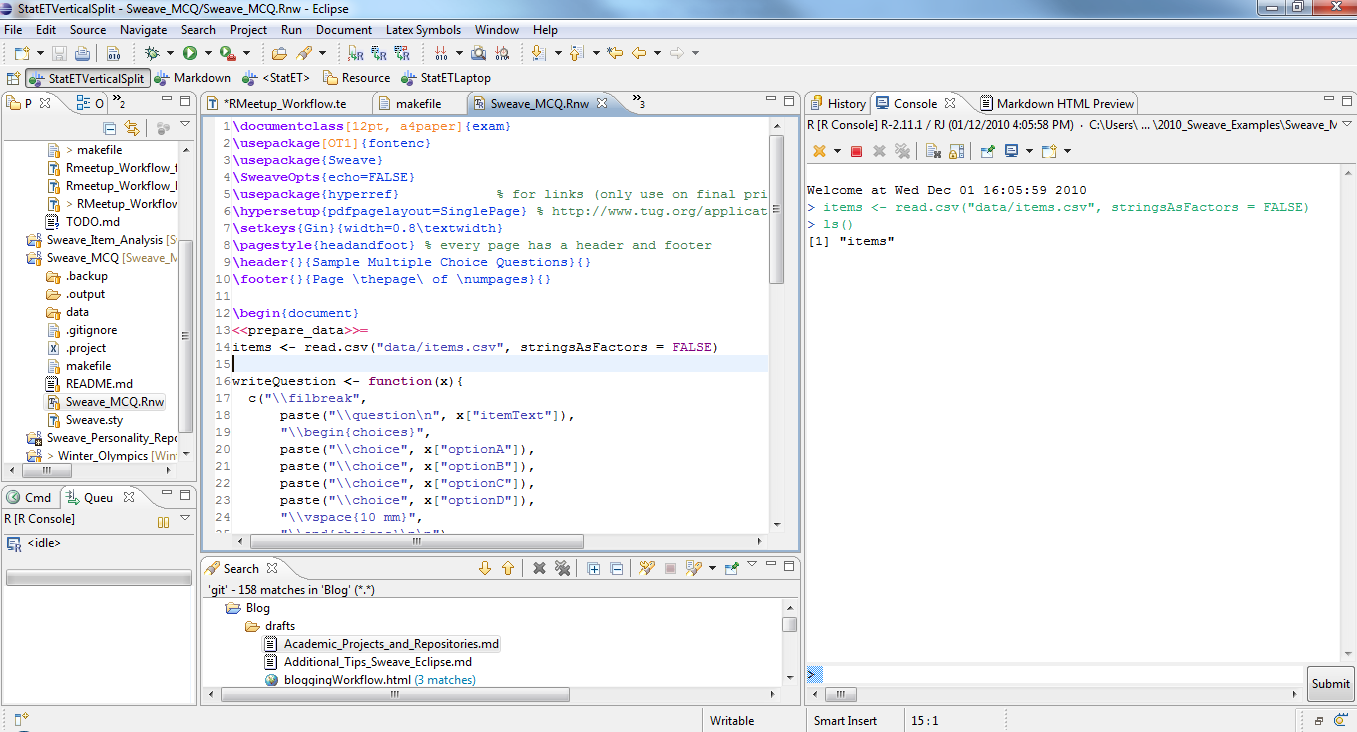
\includegraphics[width=10cm]{eclipse_screenshot}
\end{center}
\end{frame}


\begin{frame}{Eclipse and StatET: Benefits}
\begin{itemize}
  \item Good support for version control
  \item Easy to hook in external tools like sh, cmd, and make
  \item File search
  \item Allows for multiple integrated consoles
  \item Configurable multi-element display (particularly good on big monitors)
\end{itemize}
\hrule
\begin{itemize}
  \item Understands R (indentation, colour coding, code folding, outline view) 
  \item Great shortcut keys for sending R code to console and getting help
  \item Understands Sweave and LaTeX
  \item Project explorer for projects, folders, files
  \item R object explorer and content assist
  \item Command history and Queue
\end{itemize}
\end{frame}

 


\begin{frame}{Eclipse and StatET: Resources}
\begin{itemize}
  \item StatET Website: \\
  {\tiny\url{http://www.walware.de/goto/statet}}
  \item Longhow Lam's Guide: \\ 
  {\tiny \url{http://www.splusbook.com/RIntro/RCourseMaterial.html}}
  \item My Guide: \\
   {\tiny \url{http://jeromyanglim.blogspot.com/2010/02/getting-started-with-sweave-r-latex.html}}
\end{itemize}
\end{frame}


\subsection{Version Control}
\begin{frame}{Version Control: Practical Benefits}
\begin{itemize}
\item Rewind a project or a file to a previous state (encourages experimentation)
\item Provides a record of changes
\item Facilitates collaboration
\item Facilitates backup
\item Shows changes between files
\item Facilitates code sharing and reproducibility
\end{itemize}
\end{frame}

\begin{frame}{Version Control: Conceptual Benefits}
\begin{itemize}
  \item the distinction between source and derived files
  \item the nature of dependencies:
	\begin{itemize}
	\item dependencies between elements of code
	\item dependencies between files within a project
	\item and dependencies with files and programs external to the repository
	\end{itemize}
  \item the nature of a repository and how repositories should be divided
  \item the nature of committing and documenting changes and project milestones
\end{itemize}
\end{frame}

\begin{frame}{Git: A Version Control System}
\begin{itemize}
  \item Popular
  \item Github
  \item Experts (e.g., Handley Wickham, Linus Torvalds)
\end{itemize}
\end{frame}


\begin{frame}{EGit: A Git plugin for Eclipse}
\begin{itemize}
  \item Simple graphical interface integrated with Eclpise 
  \item Good for getting started with version control
\end{itemize}
{\tiny Tutorial on Getting Started: 
\url{http://jeromyanglim.blogspot.com/2010/11/getting-started-with-git-egit-eclipse.html}}
\end{frame}

\subsection{make and makefiles}
\begin{frame}{make and makefiles}
\begin{itemize}
  \item One-click build
  \item Efficient build
  \item Reliable build
  \item Separate source from derived files
  \item Clean derived files
  \item Run alternative builds
  \item Encourages clear thinking about dependencies
\end{itemize}

{\tiny Tutorial on getting started:
\url{http://jeromyanglim.blogspot.com/2010/11/makefiles-for-sweave-r-and-latex-using.html}}
\end{frame}

\begin{frame}[containsverbatim, shrink=5]{Example makefile}
\begin{verbatim}
output = .output
rnwfile = Sweave_MCQ
backup = .backup

all:
    R CMD Sweave $(rnwfile).Rnw
    -mkdir $(output)
    -cp *.sty $(output)
    -mv *.tex *.pdf *.eps $(output)
    cd $(output); texify --run-viewer --pdf $(rnwfile).tex 

clean:
    -rm $(output)/*
	
backup:
    -mkdir $(backup)
    cp $(output)/$(rnwfile).pdf $(backup)/$(rnwfile).pdf 
\end{verbatim}

\end{frame}

\subsection{Sweave and LaTeX}
\begin{frame}{Sweave}

\begin{itemize}
\item Weave S (i.e., R) code chunks with LaTeX 
in a single self-describing document.
\end{itemize}

\begin{block}{Key Benfits}
\begin{itemize}
\item Reproducibility 
\item Efficiency
\item Reliability
\item Education \& Communication
\end{itemize}
\end{block}

{\tiny 
\begin{itemize}
\item Manual: \url{http://www.stat.uni-muenchen.de/~leisch/Sweave/}
\item My guide to getting started: \url{http://jeromyanglim.blogspot.com/2010/02/getting-started-with-sweave-r-latex.html}
\end{itemize}
}
\end{frame}
% basic principle

Reproducibility: The most important reason to adopt a tool like Sweave is to make your research more reproducible. The R code sets out exactly how the raw data is transformed into publication output. The Sweave document links this R output with the final report. 
Efficiency: Statistical output is automatically incorporated into your report. There is no need to copy and paste output from your statistical analysis program into your report. If your data or analyses change, you can update your report with a single click instead of having to manually update every table and figure.
Reliability: The integration of analyses with the report reduces the chance of errors entering in through copying and pasting of statistical output into documents.
Education \& Communication: By providing data analysis code for a report, this teaches others how to do similar analyses.



\section{Sweave Examples}
\begin{frame}{Overview of Examples}
\begin{block}{Different Types of Sweave Documents}
\begin{itemize}
  \item Console Report
  \item Multiple Reports
  \item Database Driven Document
  \item Non-console Report   
\end{itemize}
\end{block}

For each example links are provided to complete copies of source code with explanation.
\end{frame}

\subsection{1. Console Report}
\begin{frame}{1. Console Report: Item Analysis}
\begin{itemize}
\item {\tiny
\url{http://jeromyanglim.blogspot.com/2010/11/sweave-tutorial-3-console-input-and.html}}
\end{itemize}
\end{frame}


\subsection{2. Multiple Reports}
\begin{frame}{2. Multiple Reports: Personality Feedback}
\begin{itemize}
\item {\tiny\url{http://jeromyanglim.blogspot.com/2010/11/sweave-tutorial-2-individual.html}}
\end{itemize}
\end{frame}

\subsection{3. Database Driven Document}
\begin{frame}{3. Database Driven Document: Multiple Choice Questions}
\begin{itemize}
\item {\tiny
\url{http://jeromyanglim.blogspot.com/2010/11/sweave-tutorial-using-sweave-r-and-make.html}}
\end{itemize}
\end{frame}



\subsection{4. Non-console Report}
\begin{frame}{4. Non-console Report: Winter Olympic Medals}
\begin{itemize}
\item {\tiny \url{https://github.com/jeromyanglim/Sweave_Winter_Olympics}}
\end{itemize}
\end{frame}







\end{document}